\documentclass[a4paper, 14pt]{extarticle}
\usepackage[english,russian]{babel}
\usepackage[T1]{fontenc}
\usepackage[utf8]{inputenc}
\usepackage{fontspec}
\usepackage{indentfirst}
\usepackage{enumitem}
\usepackage{graphicx}
\usepackage[
  left=30mm,
  right=10mm,
  top=20mm,
  bottom=20mm
]{geometry}
\usepackage{parskip}
\usepackage{titlesec}
\usepackage{xurl}
\usepackage{hyperref}
\usepackage{float}
\usepackage[
  figurename=Рисунок,
  labelsep=endash,
  justification=centering
]{caption}
\usepackage[outputdir=build, newfloat]{minted}
\usepackage{chngcntr}

\selectlanguage{russian}

\hypersetup{
  colorlinks=true,
  linkcolor=black,
  filecolor=blue,
  urlcolor=blue,
}

\renewcommand*{\labelitemi}{---}
\setmainfont{Times New Roman}
\setmonofont{JetBrains Mono}[
  SizeFeatures={Size=11},
]

\newenvironment{code}{\captionsetup{type=figure}}{}
\BeforeBeginEnvironment{code}{\bigskip}
\AfterEndEnvironment{code}{\bigskip}

\setminted{
  fontsize=\footnotesize,
}

\setlength{\parskip}{6pt}

\setlength{\parindent}{1.25cm}
\setlist[itemize]{itemsep=0em,topsep=0em,parsep=0em,partopsep=0em,leftmargin=2.0cm,wide}
\setlist[enumerate]{itemsep=0em,topsep=0em,parsep=0em,partopsep=0em,leftmargin=2.0cm,wide}

\renewcommand{\thesection}{\indent\arabic{section}.}
\renewcommand{\thesubsection}{\indent\thesection\arabic{subsection}.}
\renewcommand{\thesubsubsection}{\indent\thesubsection\arabic{subsubsection}.}

\titleformat{\section}{\normalfont\bfseries}{\thesection}{0.5em}{}
\titleformat{\subsection}{\normalfont\bfseries}{\thesubsection}{0.5em}{}
\titleformat{\subsubsection}{\normalfont\bfseries}{\thesubsubsection}{0.5em}{}

\titleformat*{\section}{\normalfont\bfseries}
\titleformat*{\subsection}{\normalfont\bfseries}
\titleformat*{\subsubsection}{\normalfont\bfseries}

\titlespacing{\section}{\parindent}{\parskip}{\parskip}
\titlespacing{\subsection}{\parindent}{\parskip}{\parskip}
\titlespacing{\subsubsection}{\parindent}{\parskip}{\parskip}

\begin{document}

\begin{titlepage}
  \vspace{0pt plus2fill}
  \noindent

  \vspace{0pt plus6fill}
  \begin{center}
    {
    \bfseries
    Министерство науки и высшего образования Российской Федерации
    {
    \scriptsize
    ФЕДЕРАЛЬНОЕ ГОСУДАРСТВЕННОЕ АВТОНОМНОЕ ОБРАЗОВАТЕЛЬНОЕ УЧРЕЖДЕНИЕ ВЫСШЕГО
    ОБРАЗОВАНИЯ
    }
    «Национальный исследовательский университет ИТМО»

    (Университет ИТМО)

    \begin{minipage}[t]{0.42\textwidth}
      \vspace*{0pt}
      \begin{flushright}
        Факультет

        Образовательная программа
      \end{flushright}
    \end{minipage}
    \begin{minipage}[t]{0.57\textwidth}
      \vspace*{0pt}
      \begin{flushright}
        Инфокоммуникационных технологий

        11.03.02 Программирование в инфокоммуникационных системах
      \end{flushright}
    \end{minipage}
    }

    \vspace{0pt plus5fill}

    \LARGE{
      ОТЧЕТ

      по лабораторной работе 7

      по дисциплине \textbf{<<Разработка баз данных>>}
    }
  \end{center}

  \vspace{0pt plus4fill}
  \begin{flushright}
    Выполнил: \textbf{студент группы K33211 Швалов Д. А.}

    Проверил: \textbf{ст. преподаватель Осетрова И.С.}
  \end{flushright}

  \vspace{0pt plus8fill}
  \begin{center}
    Санкт-Петербург

    2024
  \end{center}
\end{titlepage}

\setcounter{page}{2}

\linespread{1.5}
\renewcommand{\baselinestretch}{1.5}

\section*{\large{Лабораторная работа №7 <<Создание триггеров>>}}

\section{Цель работы}

Создание триггеров.

\section{Задачи, решаемые при выполнении работы}

\begin{enumerate}[leftmargin=*]
  \item Создание триггера DML.
  \item Создание триггера DDL.
  \item Удаление триггера DDL.
  \item Дополнительное задание 1.
  \item Дополнительное задание 2.
\end{enumerate}

\section{Объект исследования}

Создание триггеров в СУБД \foreignlanguage{english}{Microsoft SQL
  Server} с помощью \foreignlanguage{english}{Microsoft SQL Server Management
  Studio (SSMS)}.

\section{Исходные данные}

\begin{itemize}
  \item методические указания к лабораторной работе;
  \item СУБД Microsoft SQL Server;
  \item Microsoft SQL Server Management Studio;
  \item база данных ApressFinancial.
\end{itemize}

\section{Выполнение работы}

\subsection{Первая задача}

\subsubsection{Создание триггера DML}

С помощью запроса, показанного на рисунке \ref{fig:task-1-1}, был создан триггер
DML под названием <<\foreignlanguage{english}{trg\_InsTransactions}>>, который
изменяет остаток средств на счете клиента при выполнении финансовой операции (т.
е. при создании транзакции). Как видно на рисунке \ref{fig:task-1-2}, после
выполнения запроса триггер был успешно создан.

С помощью запроса, изображенного на рисунке \ref{fig:task-1-3}, был
протестирован созданный триггер. Для этого для клиента с идентификатором, равный
двум, была создана новая транзакция. Как видно на рисунке \ref{fig:task-1-4},
баланс клиента уменьшился на 200.

\begin{figure}[H]
  \centering
  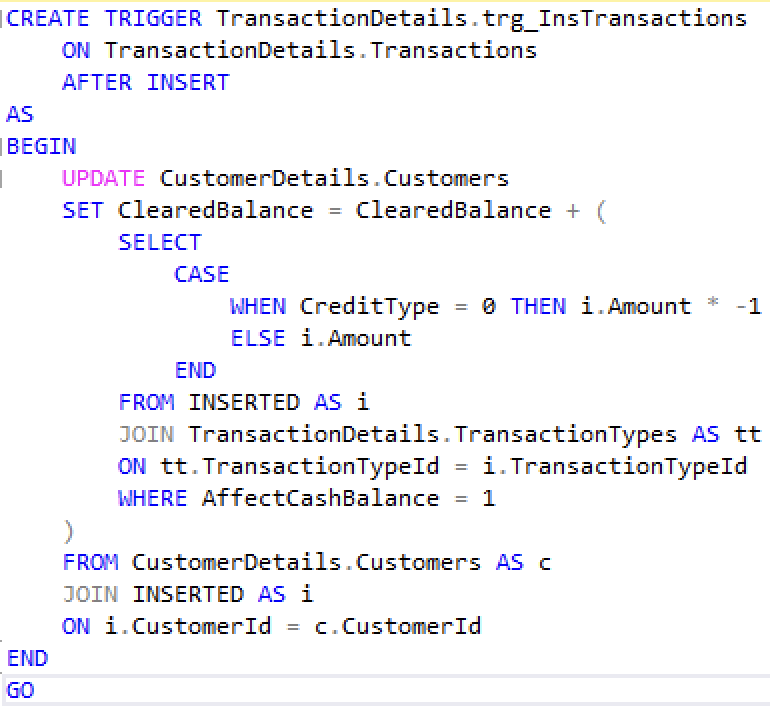
\includegraphics[width=0.7\textwidth]{images/task-1/1.png}
  \caption{
    Запрос для создания триггера
    <<\foreignlanguage{english}{trg\_InsTransactions}>>
  }
  \label{fig:task-1-1}
\end{figure}

\begin{figure}[H]
  \centering
  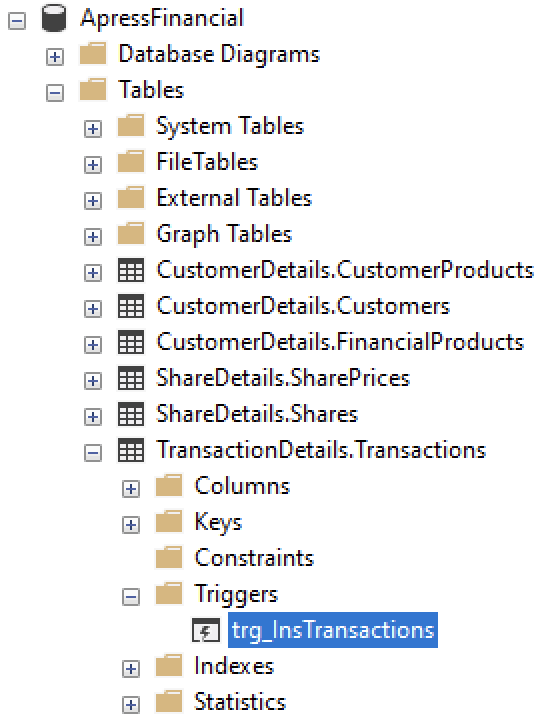
\includegraphics[width=0.5\textwidth]{images/task-1/2.png}
  \caption{Созданный триггер}
  \label{fig:task-1-2}
\end{figure}

\begin{figure}[H]
  \centering
  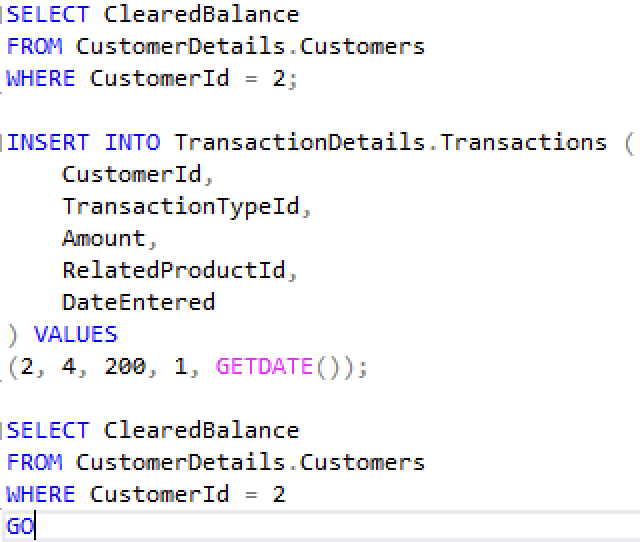
\includegraphics[width=0.6\textwidth]{images/task-1/3.png}
  \caption{Запрос для тестирования созданного триггера}
  \label{fig:task-1-3}
\end{figure}

\begin{figure}[H]
  \centering
  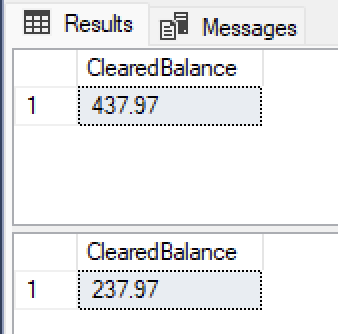
\includegraphics[width=0.5\textwidth]{images/task-1/4.png}
  \caption{Результат выполнения запроса}
  \label{fig:task-1-4}
\end{figure}

\subsubsection{Изменение триггера DML}

Триггер, созданный на предыдущем этапе, не будет работать в случае, если
транзакция не изменяет баланс клиента. Чтобы проверить это, с помощью запроса,
показанного на рисунке \ref{fig:task-1-5}, поле
<<\foreignlanguage{english}{ClearedBalance}>> было сделано обязательным. При
выполнении запроса, приведенного на рисунке \ref{fig:task-1-6}, в котором
создается транзакция, не влияющая на баланс клиента, появляется ошибка (рисунок
\ref{fig:task-1-7}).

С помощью запроса, показанного на рисунке \ref{fig:task-1-8}, созданный ранее
триггер был изменен: теперь, если подзапрос возвращает пустое значение, то
вместо него возвращается значение 0. С помощью запроса, изображенного на рисунке
\ref{fig:task-1-9}, было протестировано поведение измененного триггера. Как
видно на рисунке \ref{fig:task-1-10}, теперь запрос выполняется без ошибок и
транзакция создается.

\begin{figure}[H]
  \centering
  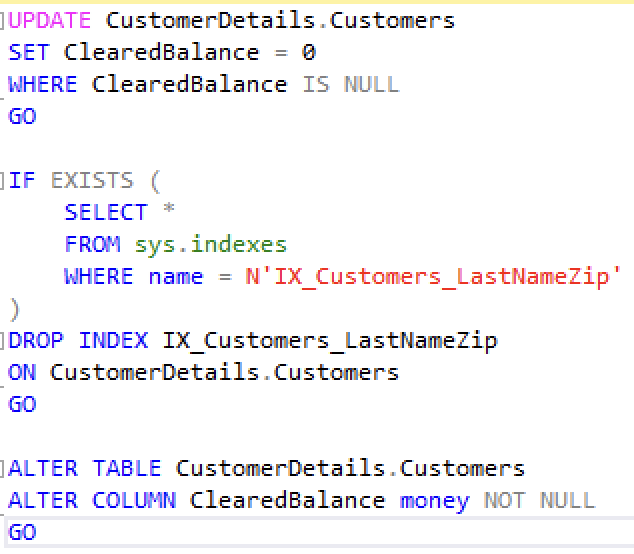
\includegraphics[width=0.6\textwidth]{images/task-1/5.png}
  \caption{
    Запрос для изменения поля <<\foreignlanguage{english}{ClearedBalance}>>
  }
  \label{fig:task-1-5}
\end{figure}

\begin{figure}[H]
  \centering
  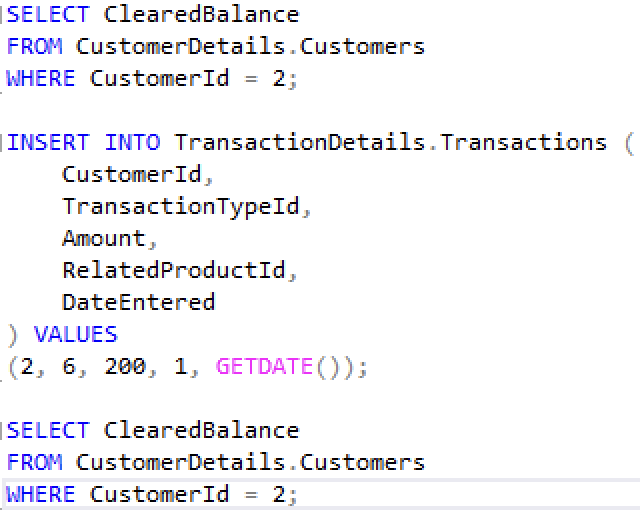
\includegraphics[width=0.6\textwidth]{images/task-1/6.png}
  \caption{Запрос для создания транзакции, не изменяющей баланс клиента}
  \label{fig:task-1-6}
\end{figure}

\begin{figure}[H]
  \centering
  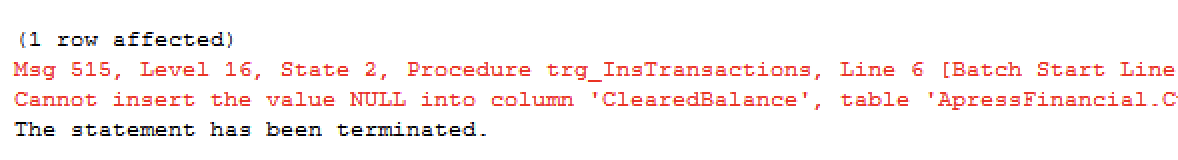
\includegraphics[width=\textwidth]{images/task-1/7.png}
  \caption{Сообщение об ошибке}
  \label{fig:task-1-7}
\end{figure}

\begin{figure}[H]
  \centering
  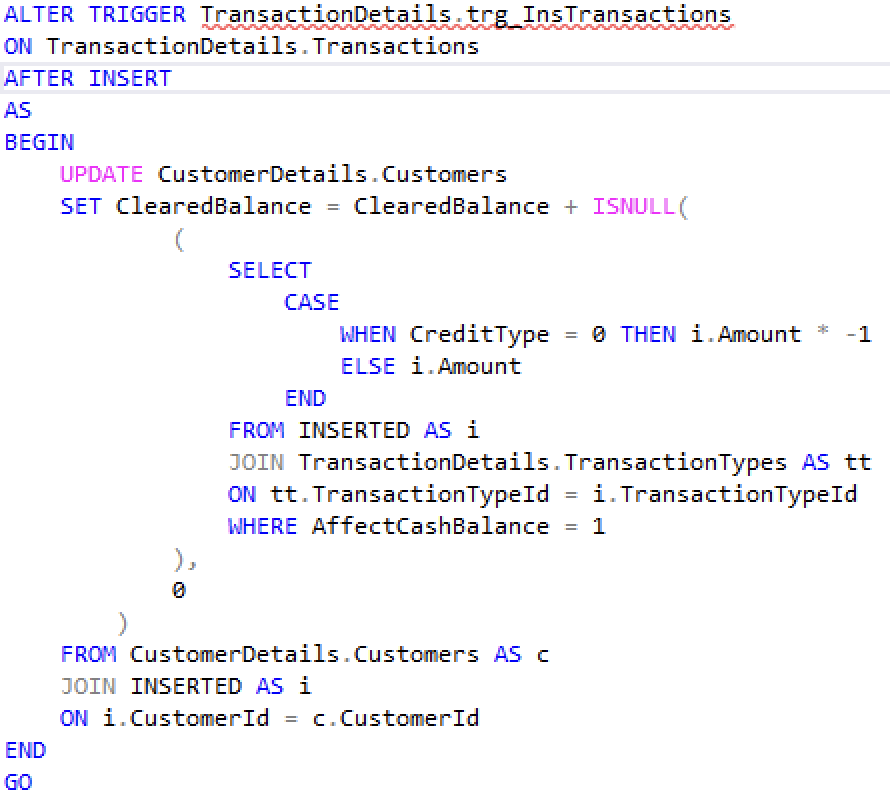
\includegraphics[width=0.8\textwidth]{images/task-1/8.png}
  \caption{Запрос для изменения триггера}
  \label{fig:task-1-8}
\end{figure}

\begin{figure}[H]
  \centering
  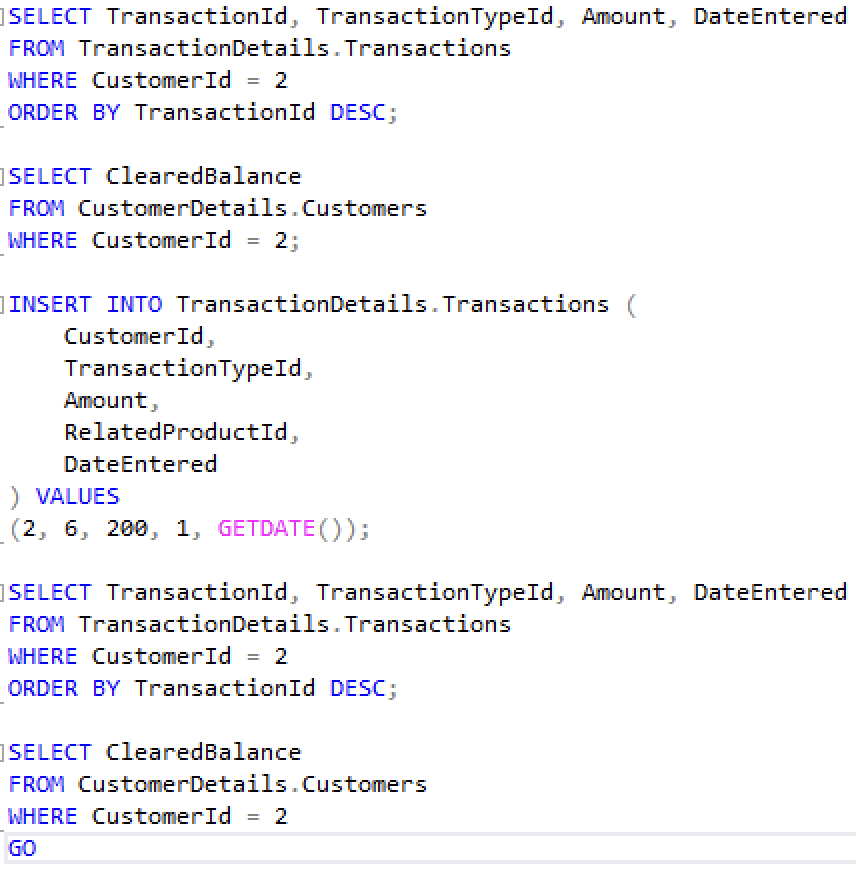
\includegraphics[width=0.8\textwidth]{images/task-1/9.png}
  \caption{Запрос для тестирования изменений}
  \label{fig:task-1-9}
\end{figure}

\begin{figure}[H]
  \centering
  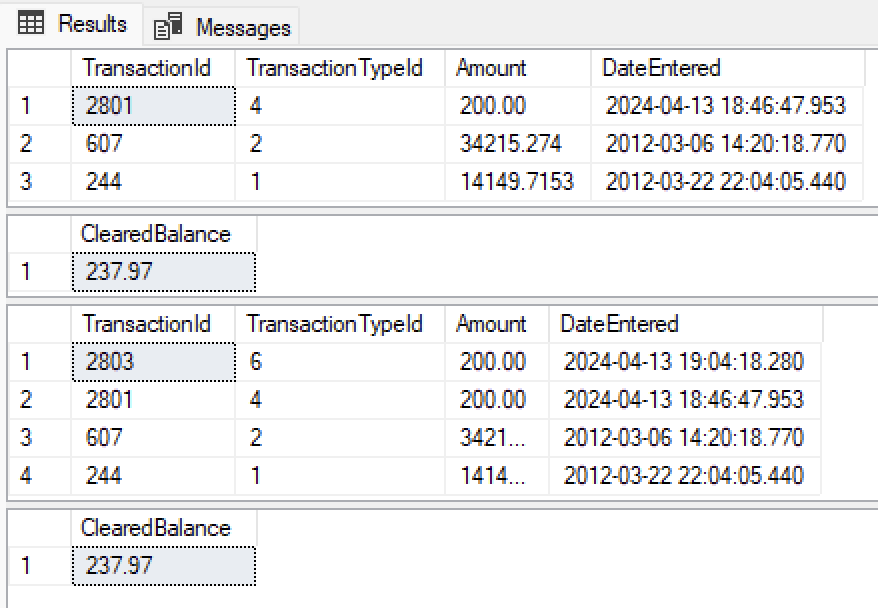
\includegraphics[width=0.7\textwidth]{images/task-1/10.png}
  \caption{Результат выполнения запроса}
  \label{fig:task-1-10}
\end{figure}

\subsection{Вторая задача}

\subsubsection{Создание триггера DDL (хранимые процедуры)}

С помощью запроса, показанного на рисунке \ref{fig:task-2-1}, был создан триггер
DDL с наименованием <<\foreignlanguage{english}{trg\_Sprocs}>>. Данный триггер
выполняется при создании хранимой процедуры и проверяет, что триггер создается в
нерабочие часы. После выполнения данного запроса новый триггер появился в
интерфейсе SSMS (рисунок \ref{fig:task-2-2}).

Чтобы протестировать созданный триггер, были выполнены два запроса. Первый,
показанный на рисунке \ref{fig:task-2-3}, был выполнен в нерабочие часы, а
потому процедура была успешно создана. Второй, изображенный на рисунке
\ref{fig:task-2-4}, был выполнен уже в рабочие часы. Из-за этого процедура не
была создана, вместо этого на указанную в триггере электронную почту было
отправлено сообщение.

\begin{figure}[H]
  \centering
  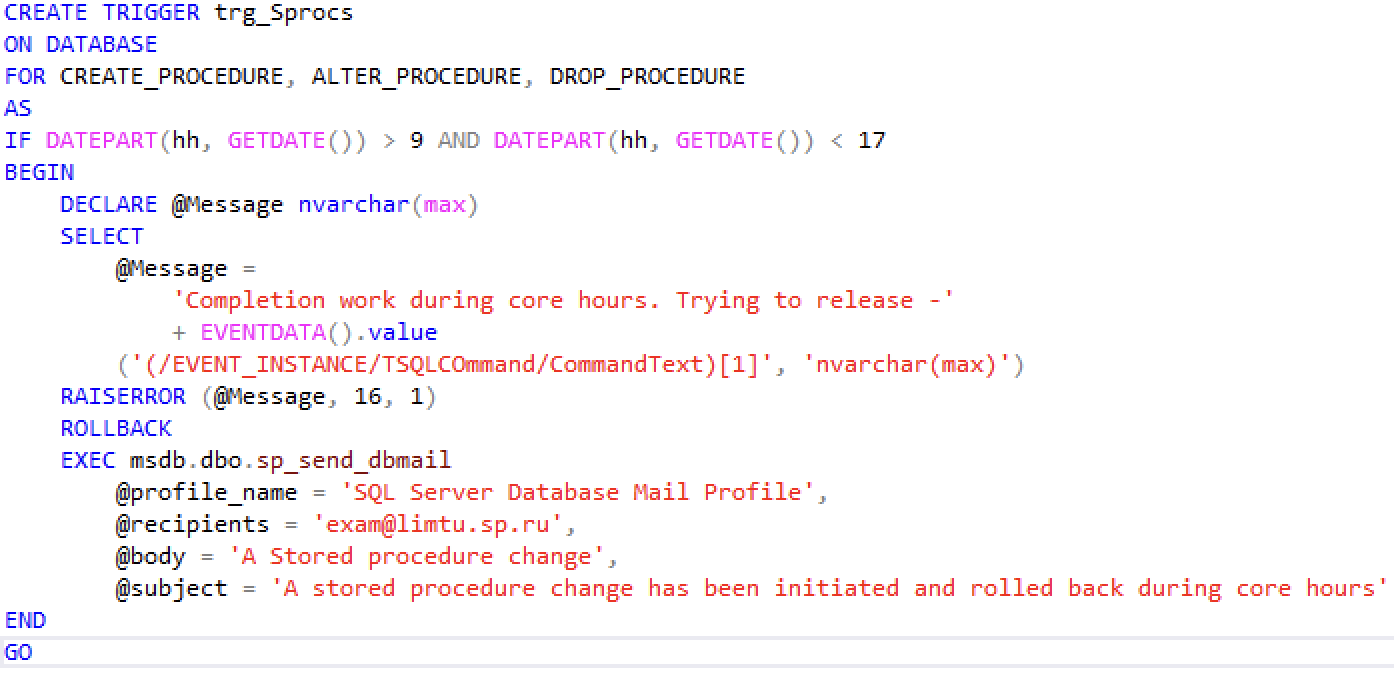
\includegraphics[width=\textwidth]{images/task-2/1.png}
  \caption{
    Запрос для создания триггера <<\foreignlanguage{english}{trg\_Sprocs}>>
  }
  \label{fig:task-2-1}
\end{figure}

\begin{figure}[H]
  \centering
  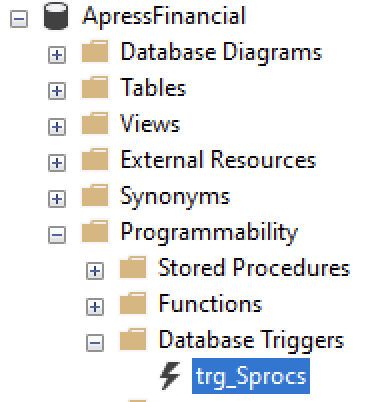
\includegraphics[width=0.3\textwidth]{images/task-2/2.png}
  \caption{Созданный триггер}
  \label{fig:task-2-2}
\end{figure}

\begin{figure}[H]
  \centering
  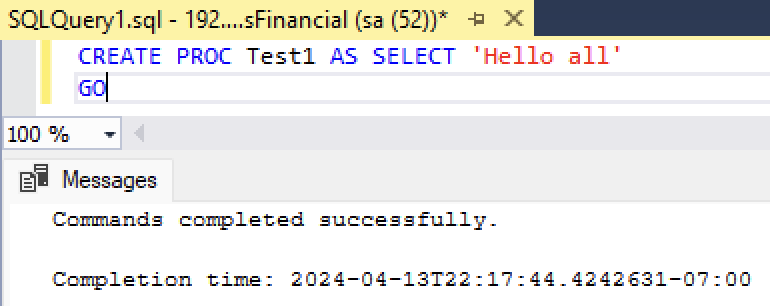
\includegraphics[width=0.8\textwidth]{images/task-2/3.png}
  \caption{Запрос для создания процедуры в нерабочие часы}
  \label{fig:task-2-3}
\end{figure}

\begin{figure}[H]
  \centering
  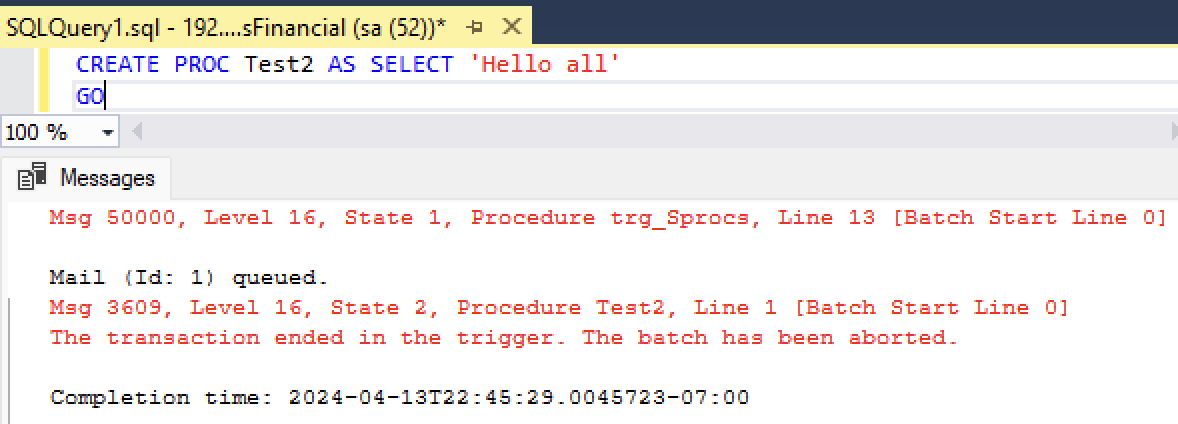
\includegraphics[width=0.8\textwidth]{images/task-2/4.png}
  \caption{Запрос для создания триггера в рабочие часы}
  \label{fig:task-2-4}
\end{figure}

\subsubsection{Создание триггера DDL (любое действие)}

С помощью запроса, показанного на рисунке \ref{fig:task-2-5}, был создан триггер
DLL под названием <<\foreignlanguage{english}{trg\_DBDump}>>, который вызывается
по любому действию, выполняемому в БД. Сам триггер выводит информацию о текущем
действии. Как показано на рисунке \ref{fig:task-2-6}, после выполнения запроса
триггер был успешно создан.

С помощью запроса, показанного на рисунке \ref{fig:task-2-7}, был протестирован
созданный триггер. При выполнении данного запроса выводится сообщение с ссылкой
на произошедшее событие. При нажатии левой кнопкой мыши на данную ссылку,
открывается подробное описание события (рисунок \ref{fig:task-2-8}).

\begin{figure}[H]
  \centering
  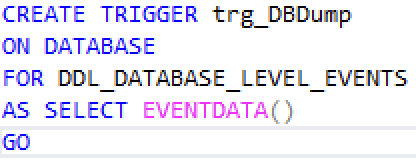
\includegraphics[width=0.5\textwidth]{images/task-2/5.png}
  \caption{
    Запрос для создания триггера <<\foreignlanguage{english}{trg\_DBDump}>>
  }
  \label{fig:task-2-5}
\end{figure}

\begin{figure}[H]
  \centering
  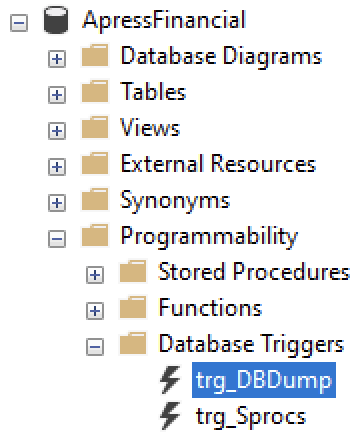
\includegraphics[width=0.4\textwidth]{images/task-2/6.png}
  \caption{Созданный триггер}
  \label{fig:task-2-6}
\end{figure}

\begin{figure}[H]
  \centering
  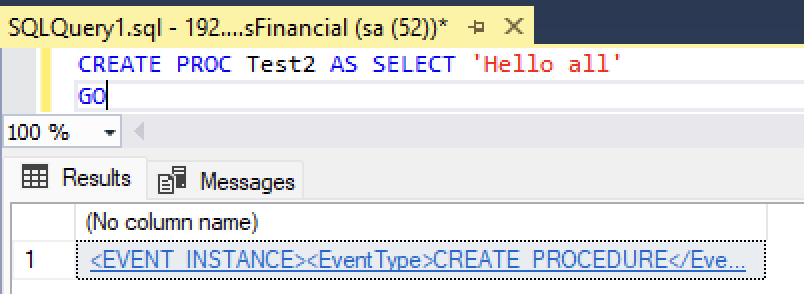
\includegraphics[width=0.8\textwidth]{images/task-2/7.png}
  \caption{Запрос для тестирования созданного триггера}
  \label{fig:task-2-7}
\end{figure}

\begin{figure}[H]
  \centering
  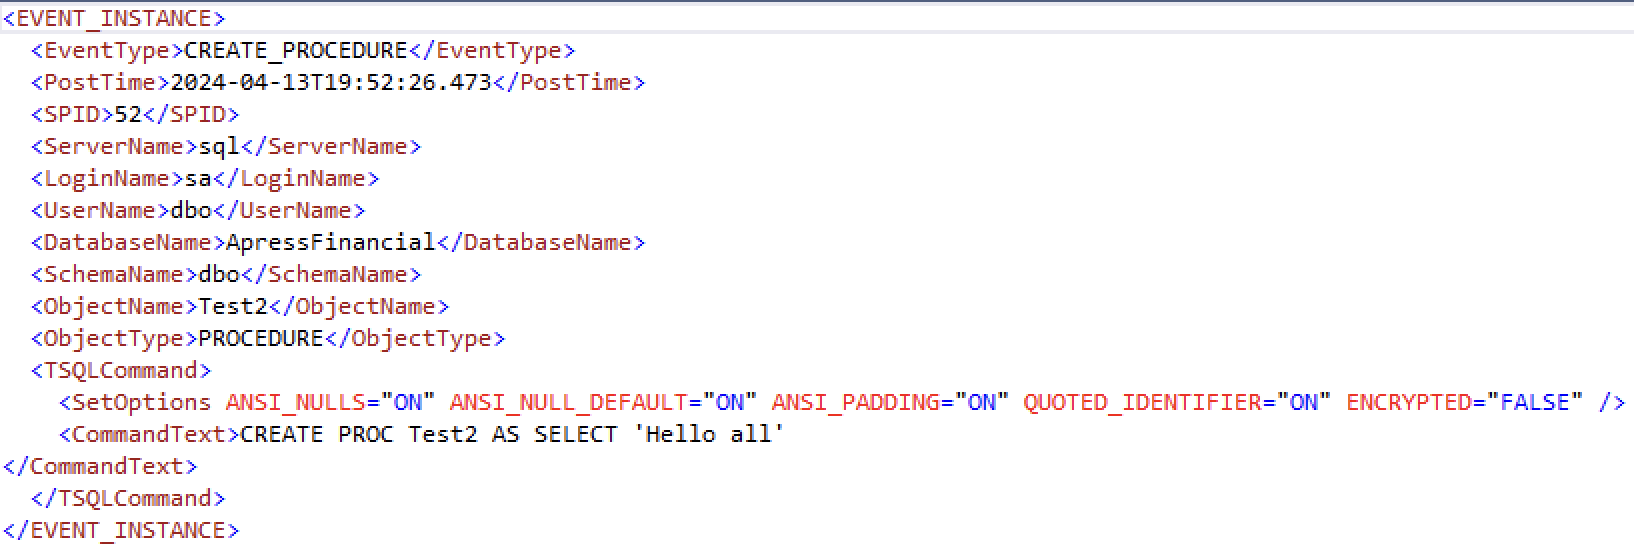
\includegraphics[width=\textwidth]{images/task-2/8.png}
  \caption{Информация о событии}
  \label{fig:task-2-8}
\end{figure}

\subsection{Третья задача}

\subsubsection{Удаление созданных триггеров и процедур}

С помощью запросов, показанный на рисунках \ref{fig:task-3-1} и
\ref{fig:task-3-2}, были удалены созданные триггеры и процедуры. После
выполнения данных запросов триггеры исчезли из интерфейса SSMS.

\begin{figure}[H]
  \centering
  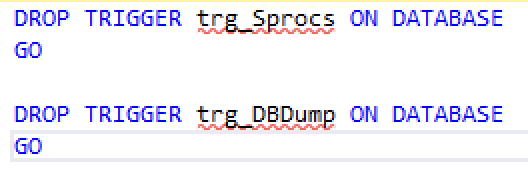
\includegraphics[width=0.7\textwidth]{images/task-3/1.png}
  \caption{Запрос для удаления созданных триггеров}
  \label{fig:task-3-1}
\end{figure}

\begin{figure}[H]
  \centering
  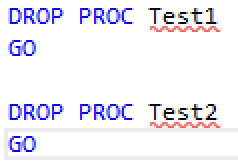
\includegraphics[width=0.4\textwidth]{images/task-3/2.png}
  \caption{Запрос для удаления созданных процедур}
  \label{fig:task-3-2}
\end{figure}

\subsection{Четвертая задача}

\subsubsection{Дополнительное задание №1}

С помощью запроса, показанного на рисунке \ref{fig:task-4-1}, созданный в
предыдущих заданиях триггер был изменен. Теперь триггер
<<\foreignlanguage{english}{trg\_InsTrasnactions}>> работает не только при
создании транзакции, но и при изменении. Однако, согласно условию данного
задания, триггер пока что не изменяет данные, если произошло обновление уже
существующей транзакции.

С помощью запросов, показанных на рисунках \ref{fig:task-4-2} и
\ref{fig:task-4-3}, было протестировано поведение измененного триггера. Как
видно на рисунках, при создании транзакции триггер изменяет данные, а при
обновлении --- нет.

\begin{figure}[H]
  \centering
  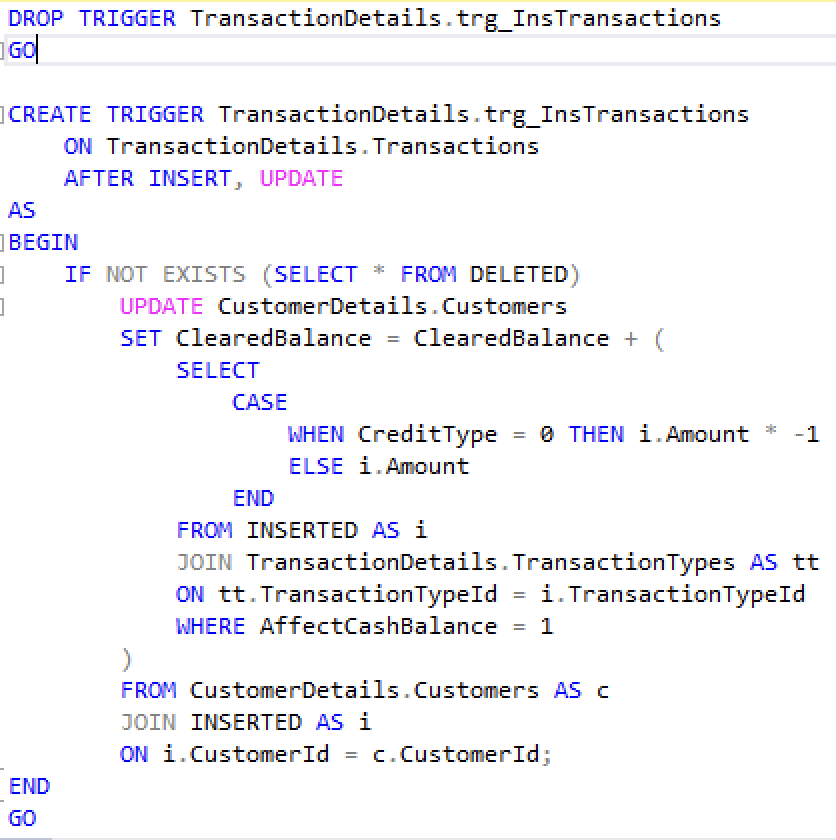
\includegraphics[width=0.8\textwidth]{images/task-4/1.png}
  \caption{
    Запрос для изменения триггера
    \foreignlanguage{english}{trg\_InsTransactions}
  }
  \label{fig:task-4-1}
\end{figure}

\begin{figure}[H]
  \centering
  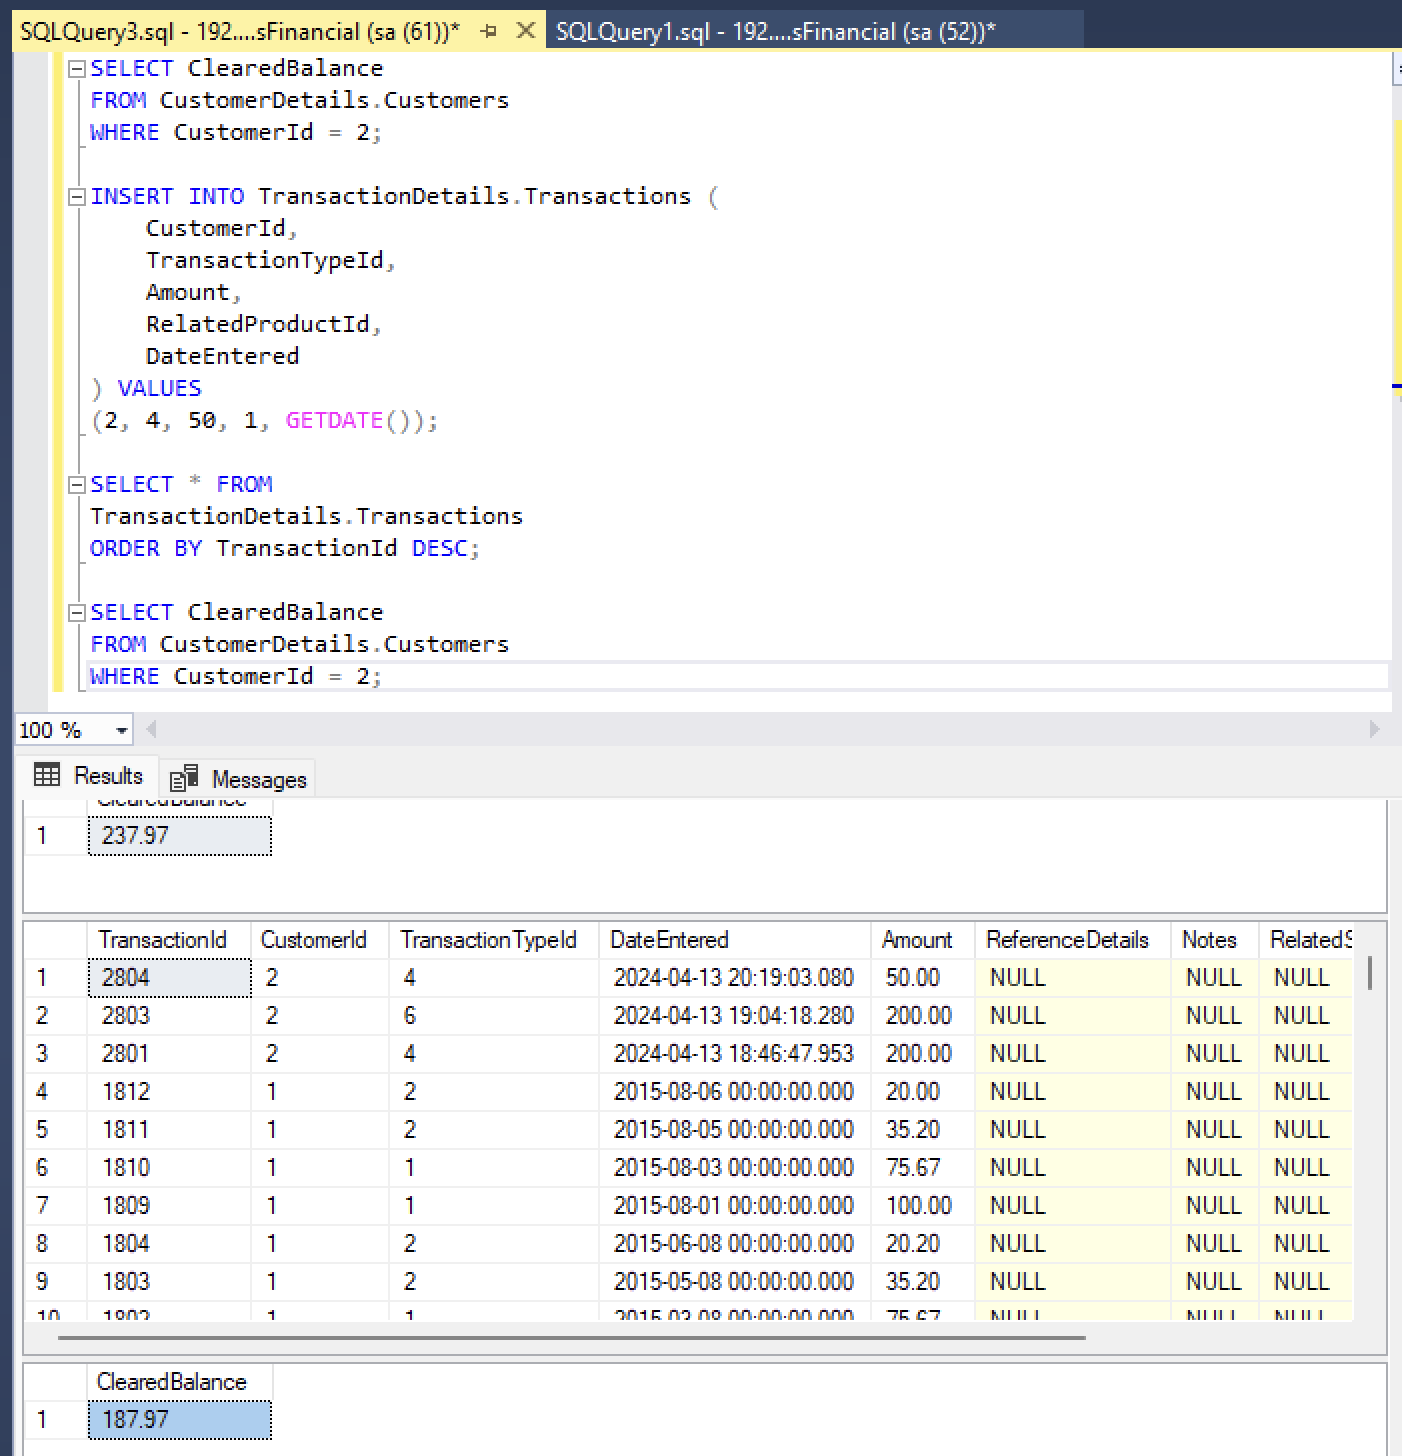
\includegraphics[width=\textwidth]{images/task-4/2.png}
  \caption{Запрос с созданием транзакции}
  \label{fig:task-4-2}
\end{figure}

\begin{figure}[H]
  \centering
  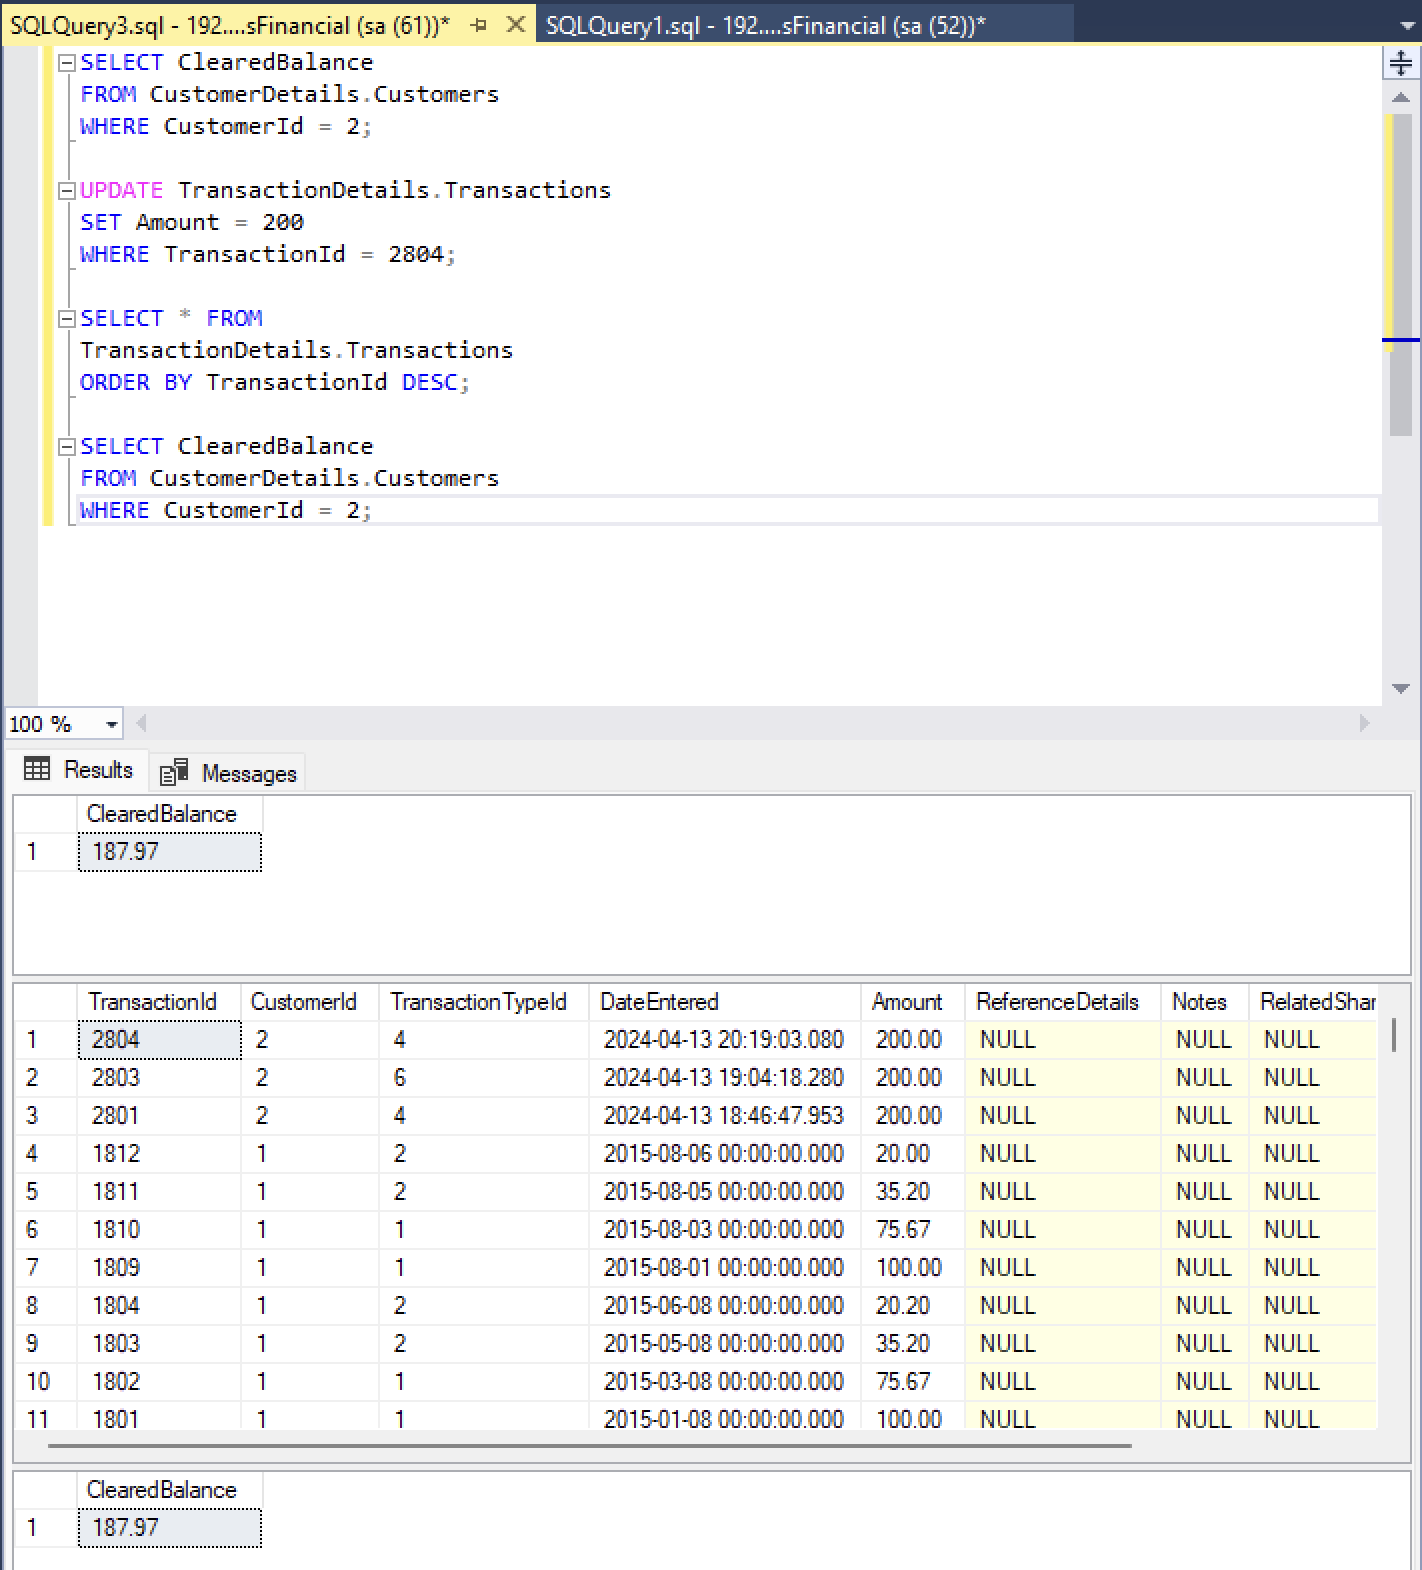
\includegraphics[width=\textwidth]{images/task-4/3.png}
  \caption{Запрос с изменением транзакции}
  \label{fig:task-4-3}
\end{figure}

\newpage

\subsection{Пятая задача}

\subsubsection{Дополнительное задание №2}

С помощью запроса, показанного на рисунке \ref{fig:task-5-1}, измененный триггер
был дополнен. Теперь баланс клиента меняется не только в случае, если была
создана новая транзакция, но и в случае, если было изменено либо поле
<<\foreignlanguage{english}{Amount}>>, либо поле
<<\foreignlanguage{english}{TransactionTypeId}>>. Также были добавлены
сообщения, которые выводится в зависимости от того, был ли изменен баланс
клиента или нет.

Как видно на рисунке \ref{fig:task-5-2}, при выполнении изменений одного из этих
полей баланс клиента меняется, а при изменении другого поля баланс остается
прежним. При этом, как изображено на рисунке \ref{fig:task-5-3}, выводится
сообщение об изменении или об отсутствии изменения.

\begin{figure}[H]
  \centering
  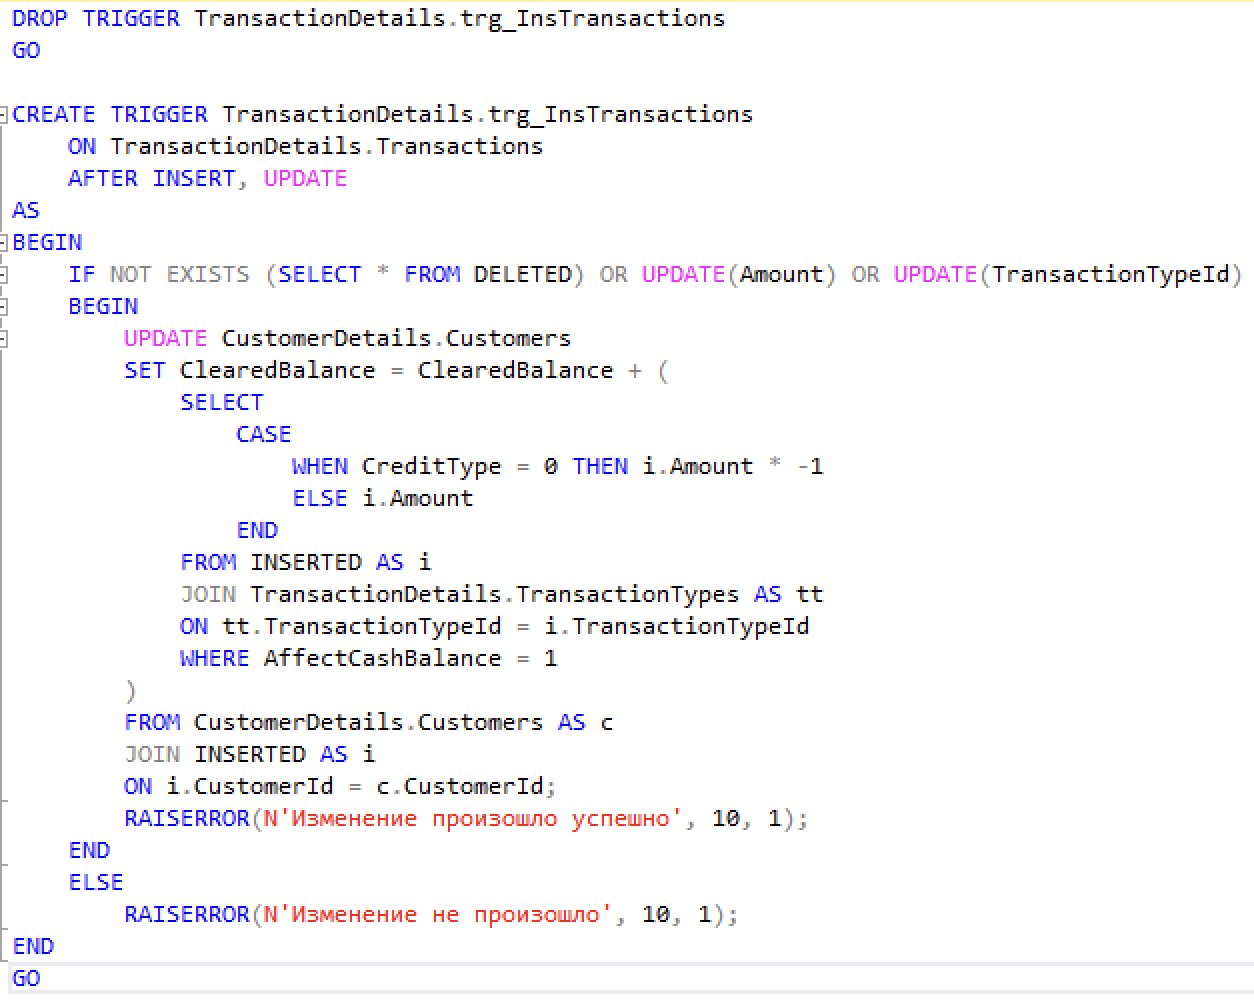
\includegraphics[width=\textwidth]{images/task-5/1.png}
  \caption{
    Запрос для изменения триггера
    \foreignlanguage{english}{trg\_InsTransactions}
  }
  \label{fig:task-5-1}
\end{figure}

\begin{figure}[H]
  \centering
  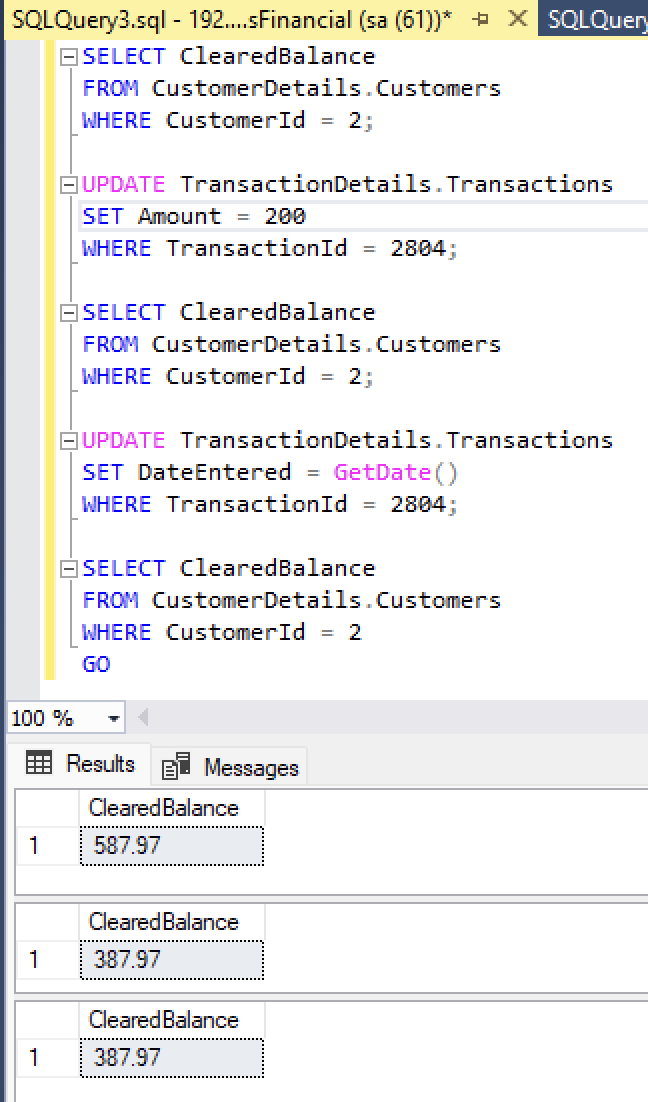
\includegraphics[width=0.5\textwidth]{images/task-5/2.png}
  \caption{Запрос с изменением транзакций}
  \label{fig:task-5-2}
\end{figure}

\begin{figure}[H]
  \centering
  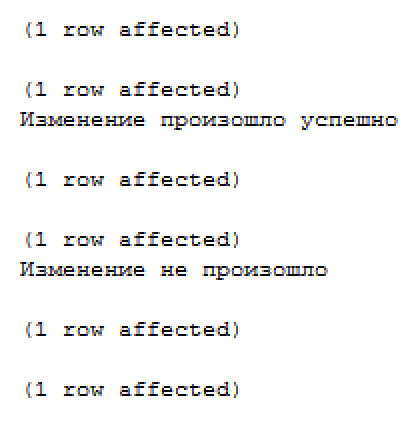
\includegraphics[width=0.4\textwidth]{images/task-5/3.png}
  \caption{Сообщения при изменении транзакций}
  \label{fig:task-5-3}
\end{figure}

\section{Выводы и анализ результатов работы}

В данной лабораторной работе изучены способы создания триггеров в SSMS. При
выполнении лабораторной работы были созданы два типа триггеров: DML и DDL. При
создании данных триггеров были рассмотрены различные события, для которых можно
создать тот или иной триггер (создание новой строки в таблице, изменение таблиц
и т. п.). Как было показано, триггеры являются очень удобным и необходимым
инструментом для создания эффективных и качественных систем хранения данных. Без
триггеров работа с базой данных была бы куда сложнее и менее безопасной.

Цель, поставленная в начале работы, достигнута, задачи выполнены.

\end{document}
